
% ---- Auto-generated LaTeX figure includes ----

\begin{figure}[t]
\centering
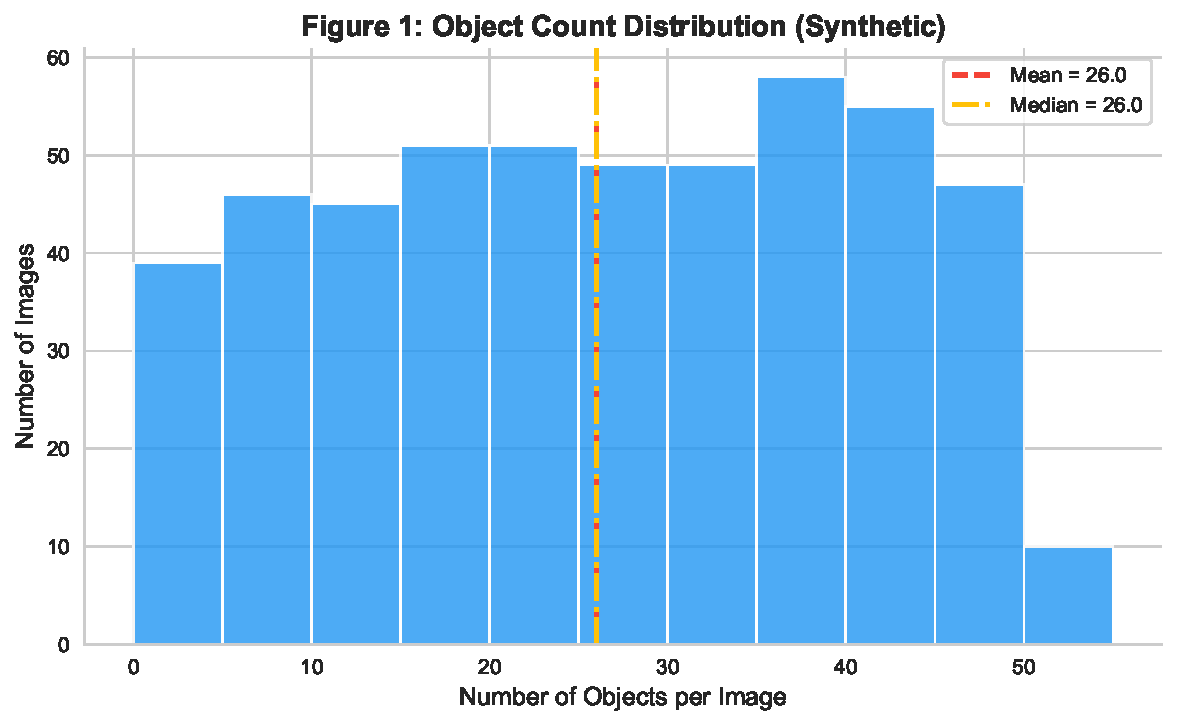
\includegraphics[width=\linewidth]{figures/fig1_object_count_distribution.pdf}
\caption{Object count distribution for the synthetic dataset.}
\label{fig:obj_count}
\end{figure}

\begin{figure}[t]
\centering
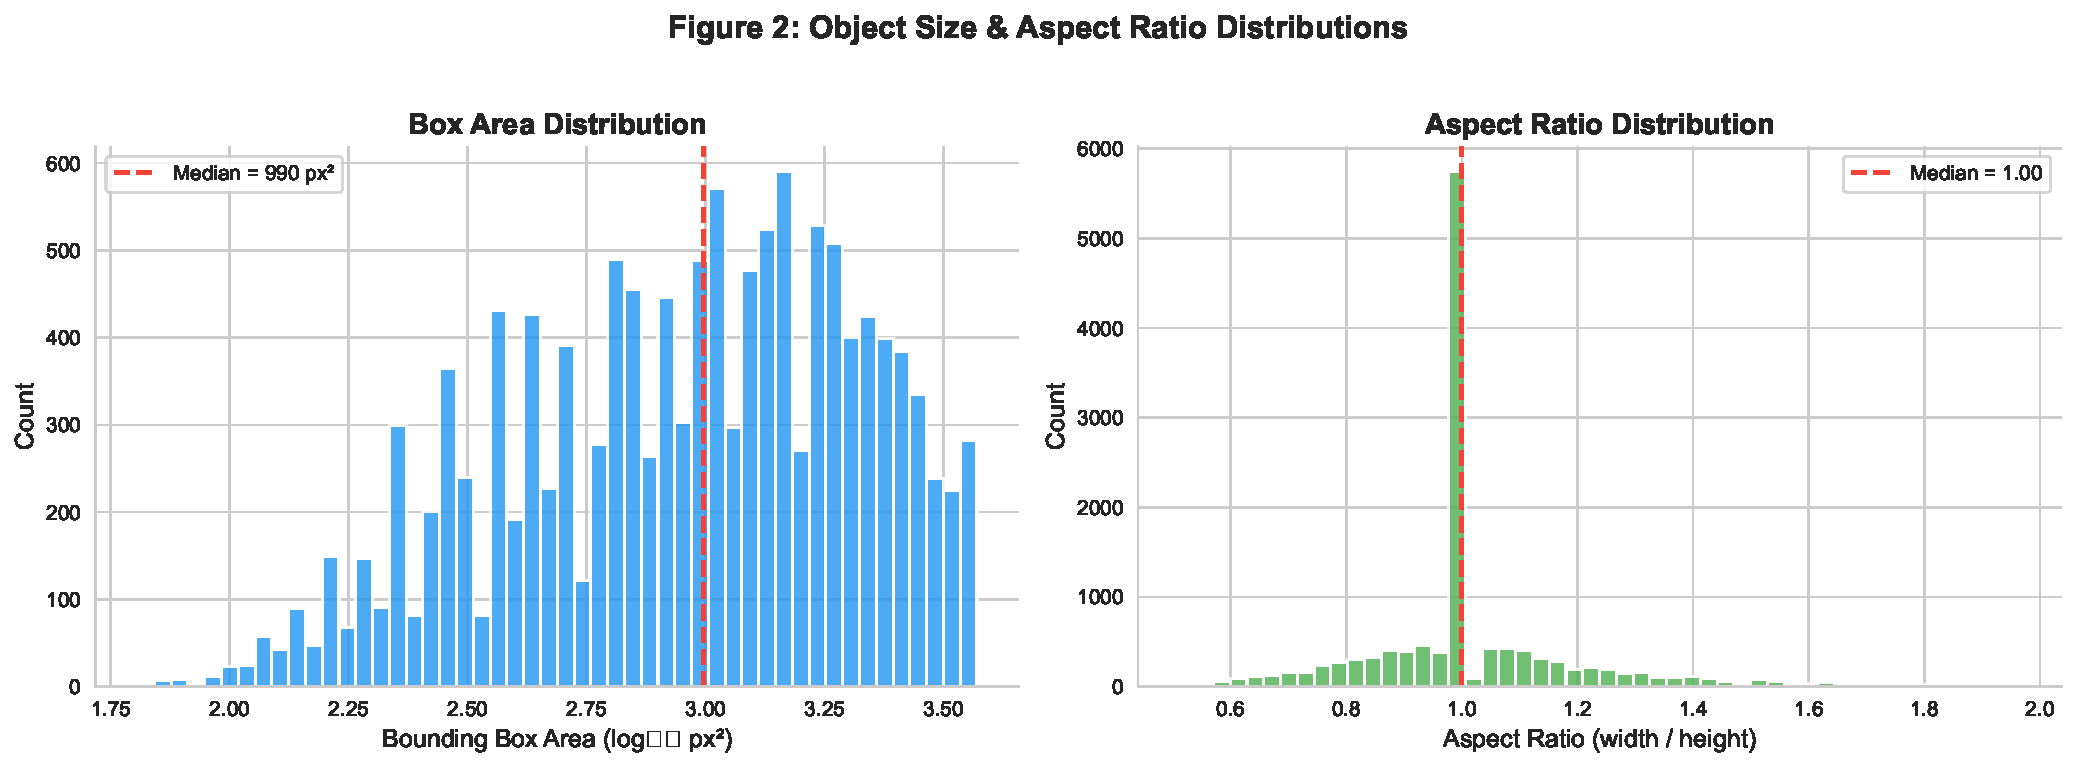
\includegraphics[width=\linewidth]{figures/fig2_size_distributions.pdf}
\caption{Bounding box area and aspect ratio distributions.}
\label{fig:size_dist}
\end{figure}

\begin{figure}[t]
\centering
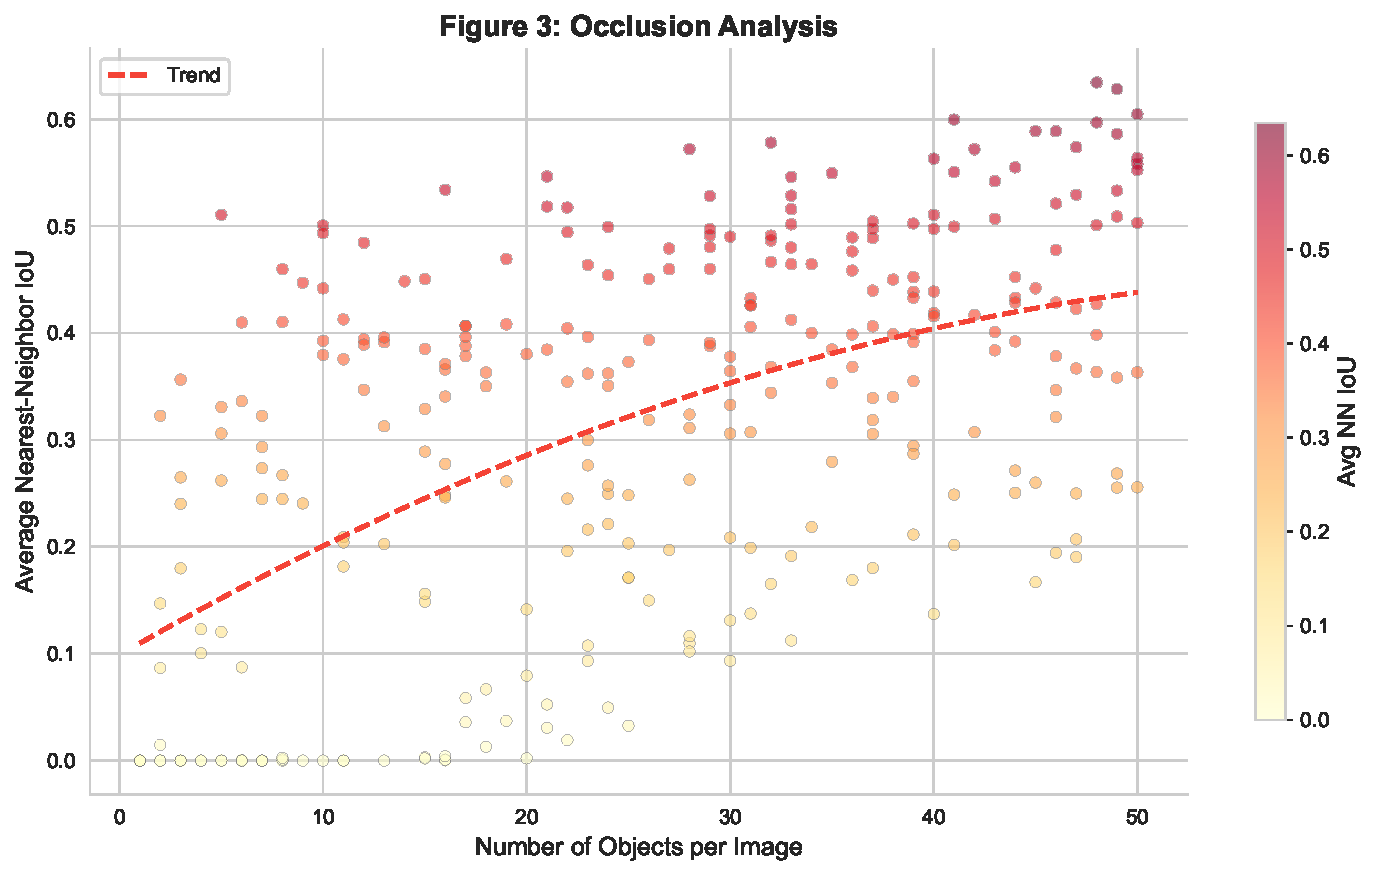
\includegraphics[width=\linewidth]{figures/fig3_occlusion_analysis.pdf}
\caption{Average nearest-neighbor IoU vs.\ number of objects.}
\label{fig:occlusion}
\end{figure}

\begin{figure}[t]
\centering
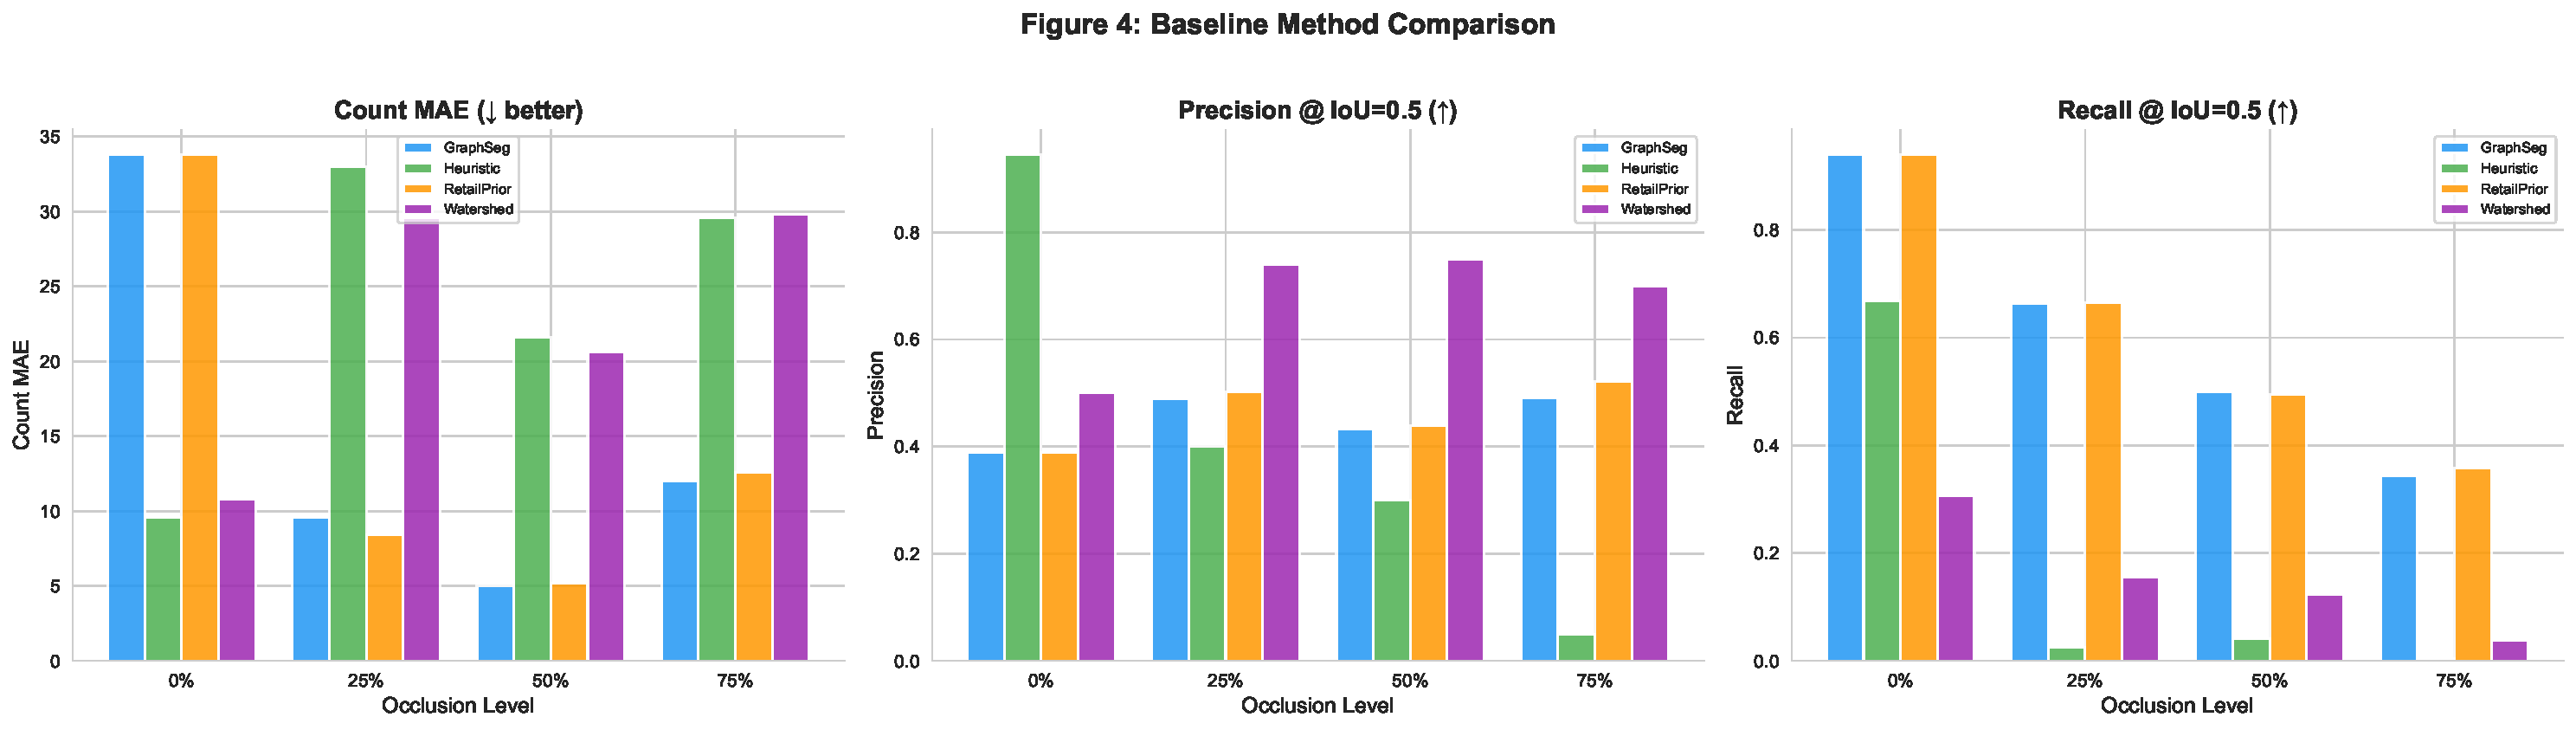
\includegraphics[width=\linewidth]{figures/fig4_baseline_comparison.pdf}
\caption{Count MAE, Precision, and Recall across classical methods.}
\label{fig:baseline_comp}
\end{figure}

\begin{figure}[t]
\centering
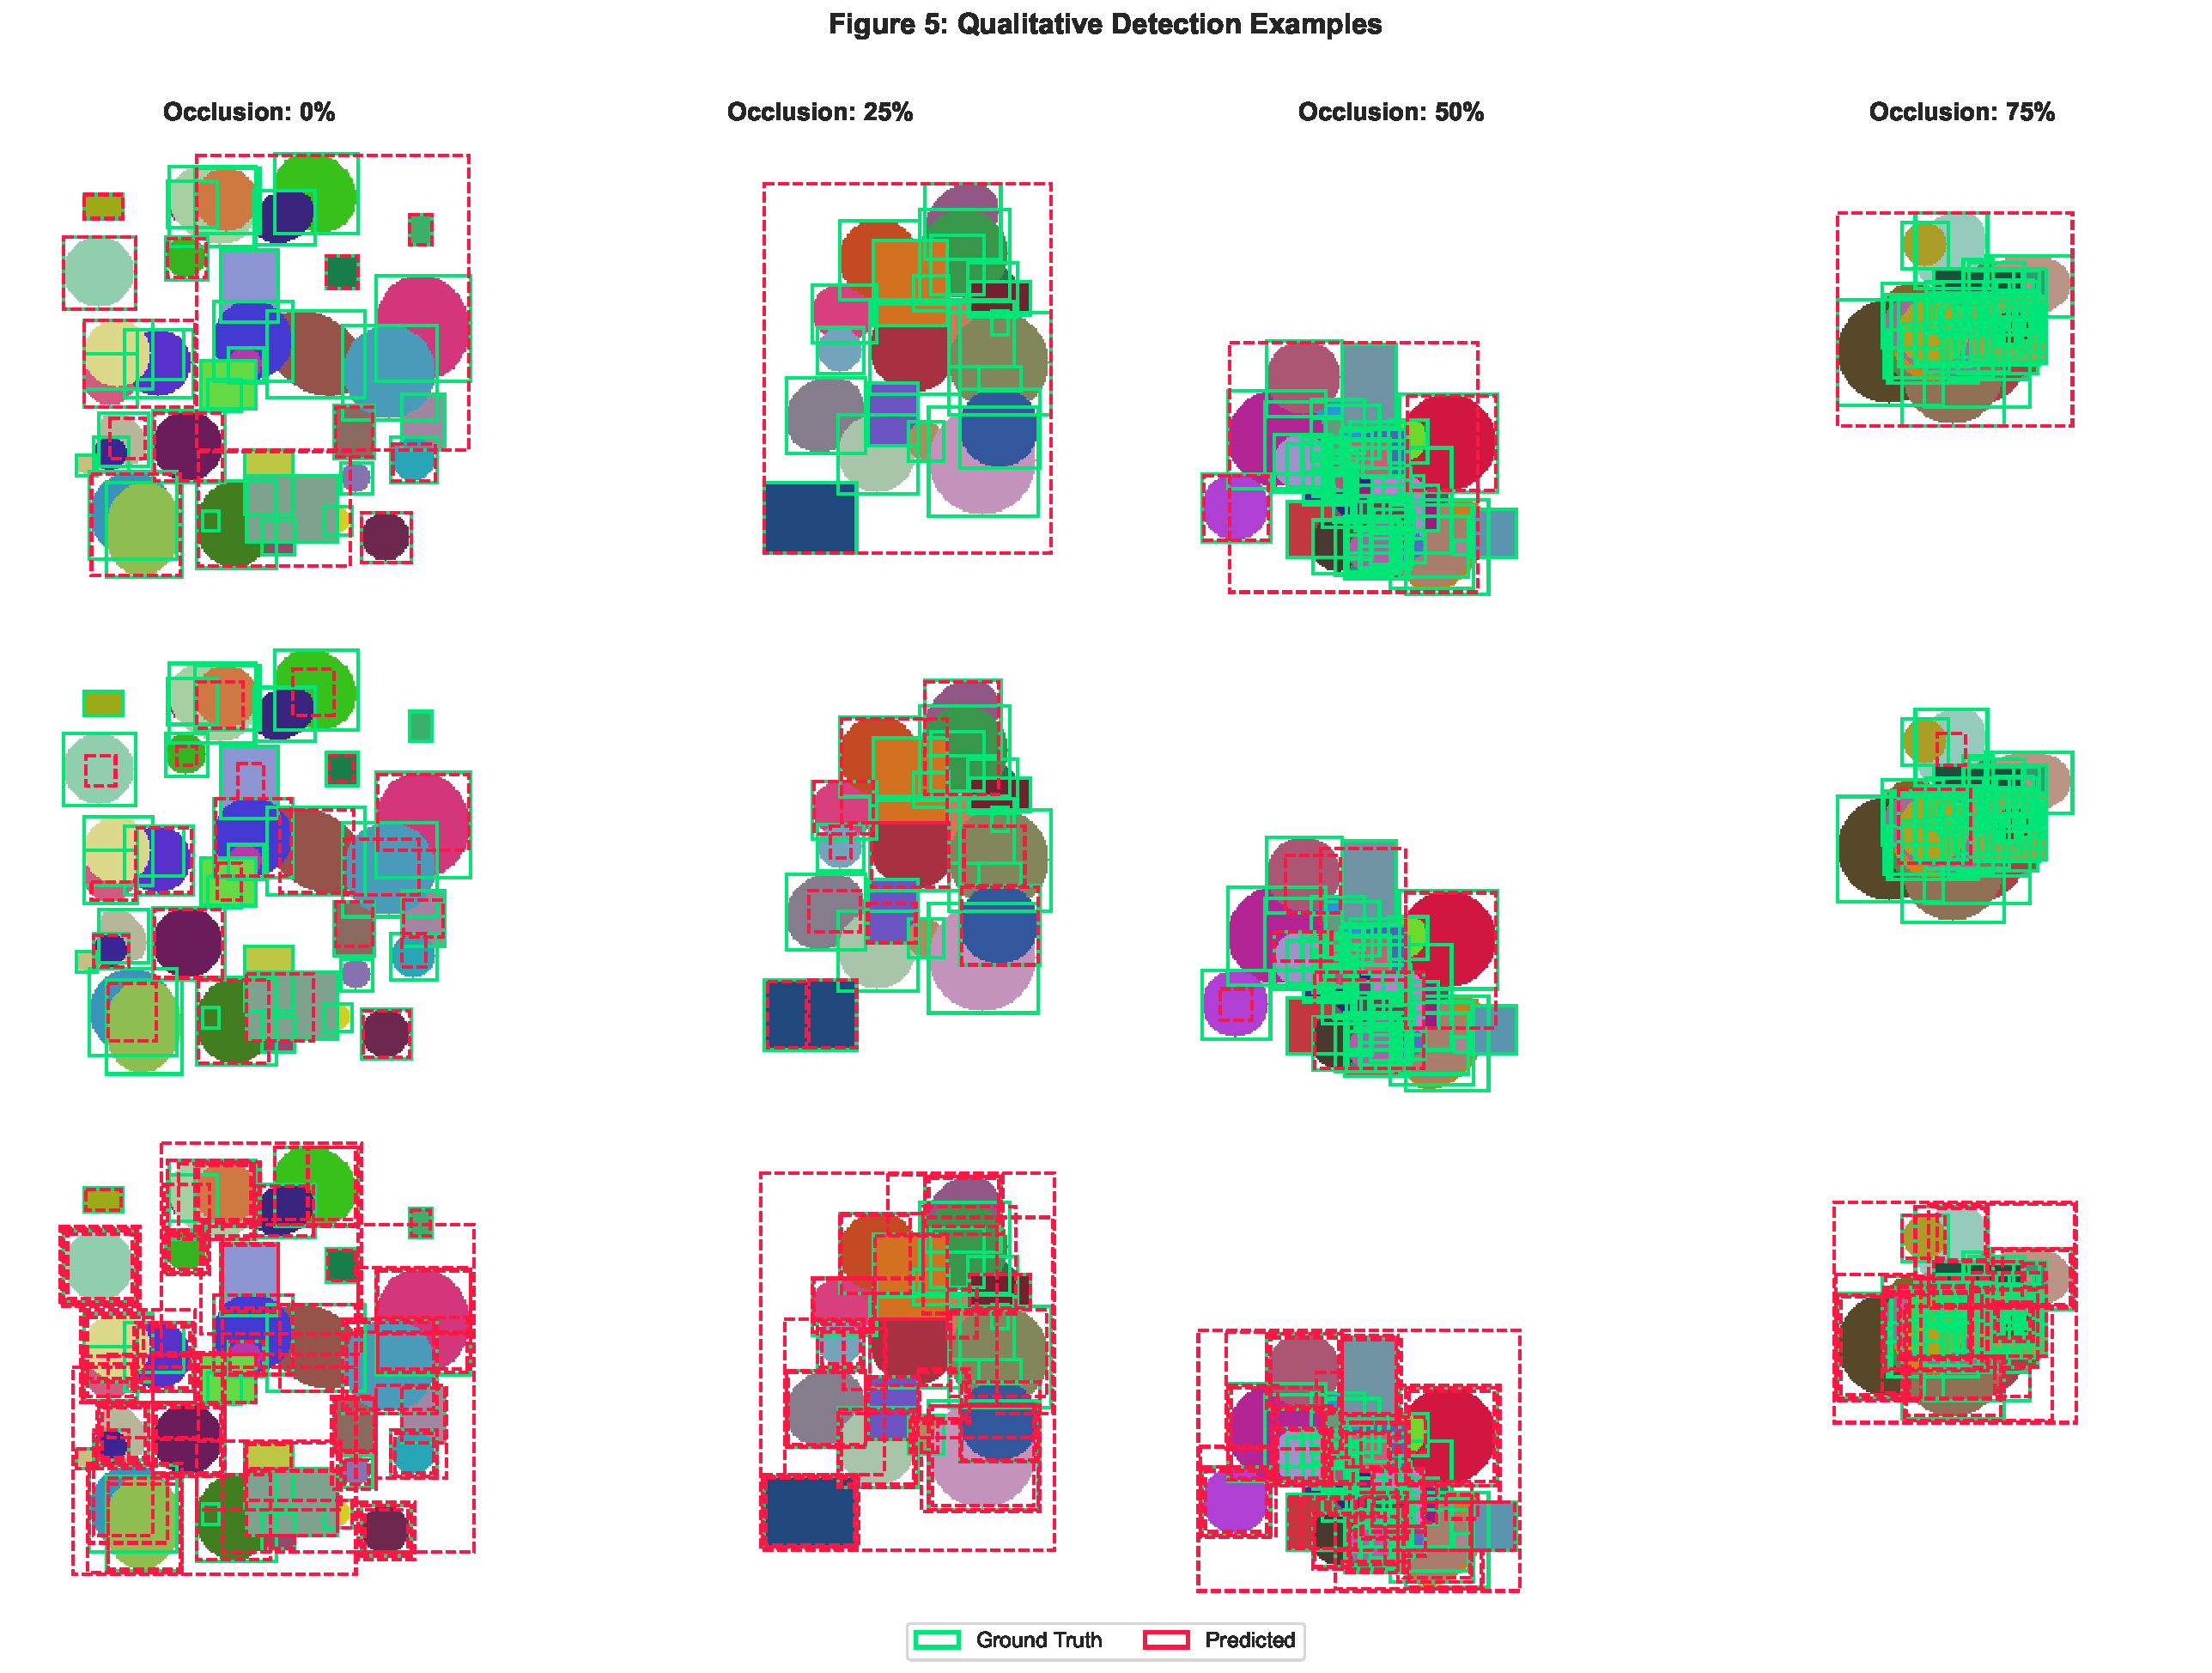
\includegraphics[width=\linewidth]{figures/fig5_detection_grid.pdf}
\caption{Qualitative detection examples: methods vs.\ occlusion levels.}
\label{fig:det_grid}
\end{figure}

\begin{figure}[t]
\centering
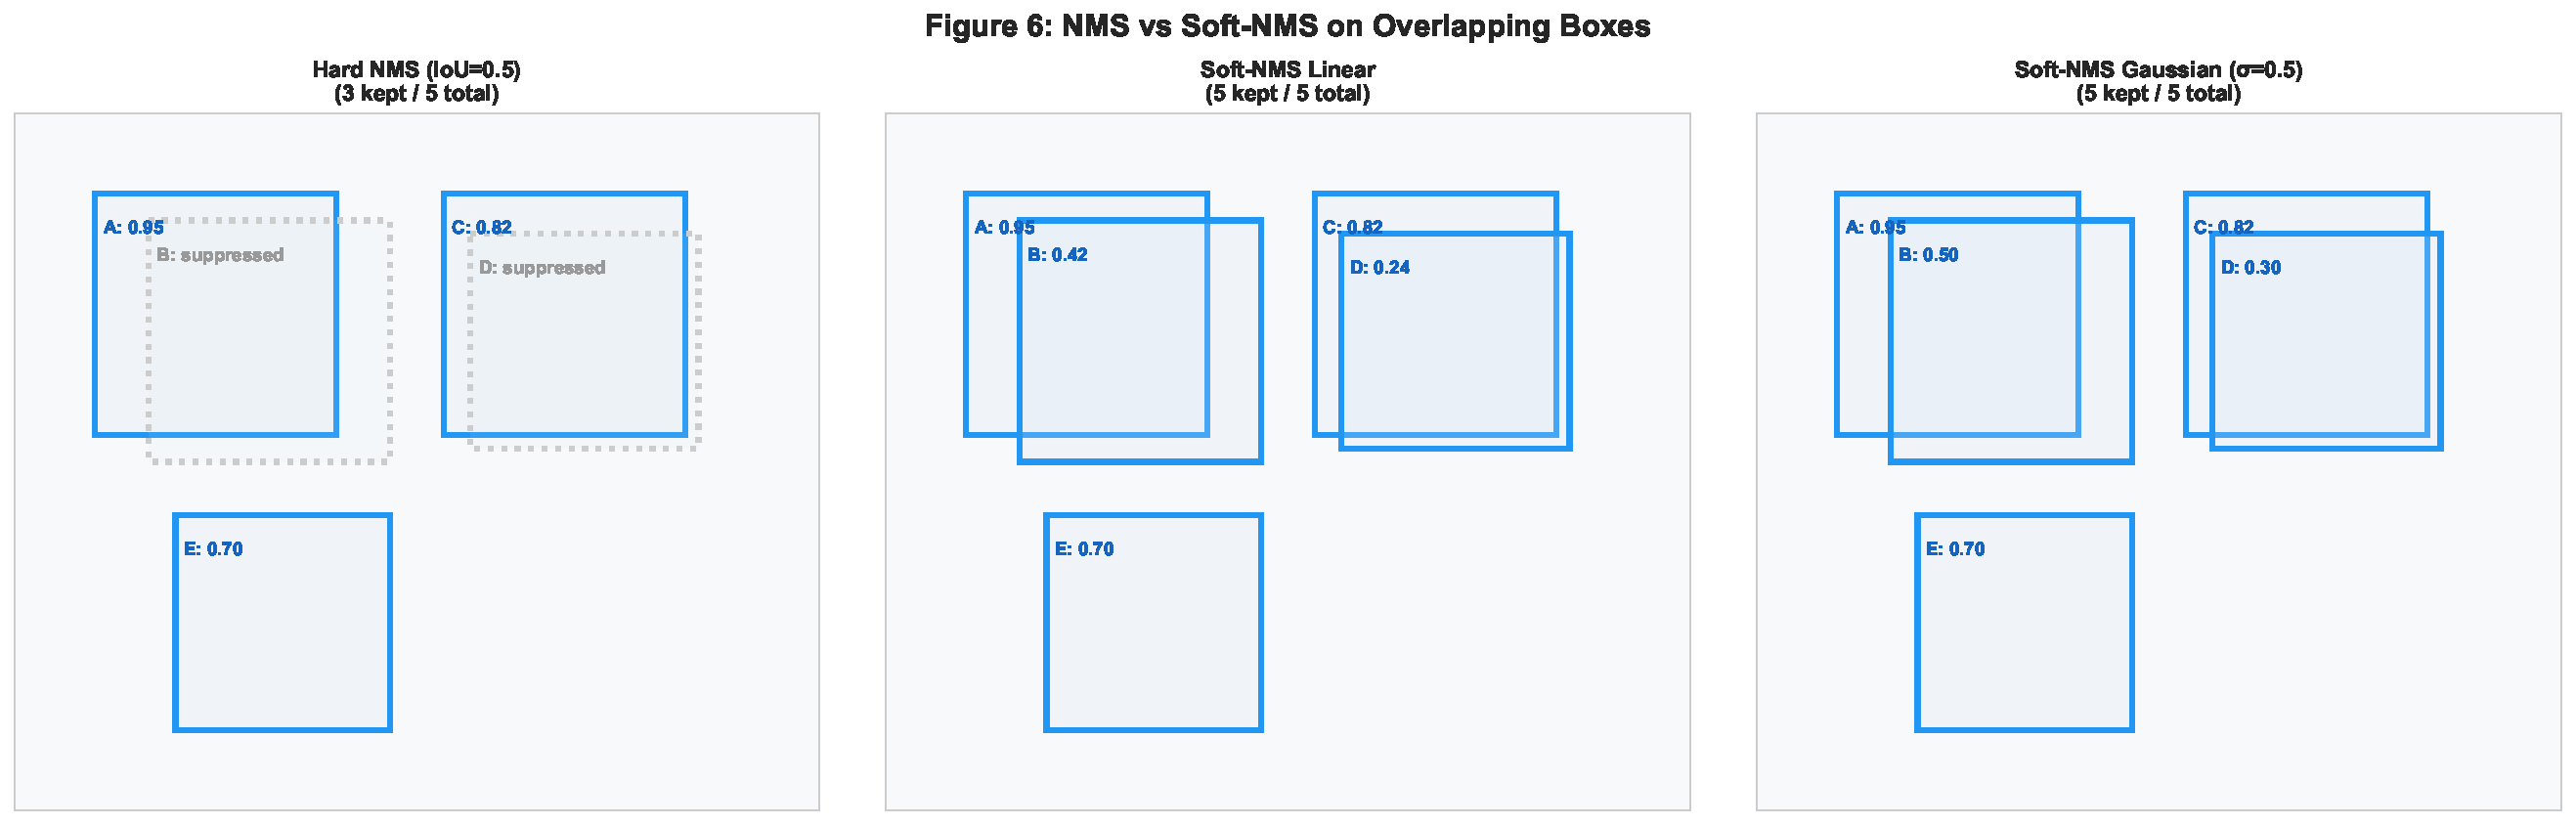
\includegraphics[width=\linewidth]{figures/fig6_nms_comparison.pdf}
\caption{Hard NMS vs.\ Soft-NMS score decay on overlapping boxes.}
\label{fig:nms_comp}
\end{figure}

\begin{figure}[t]
\centering
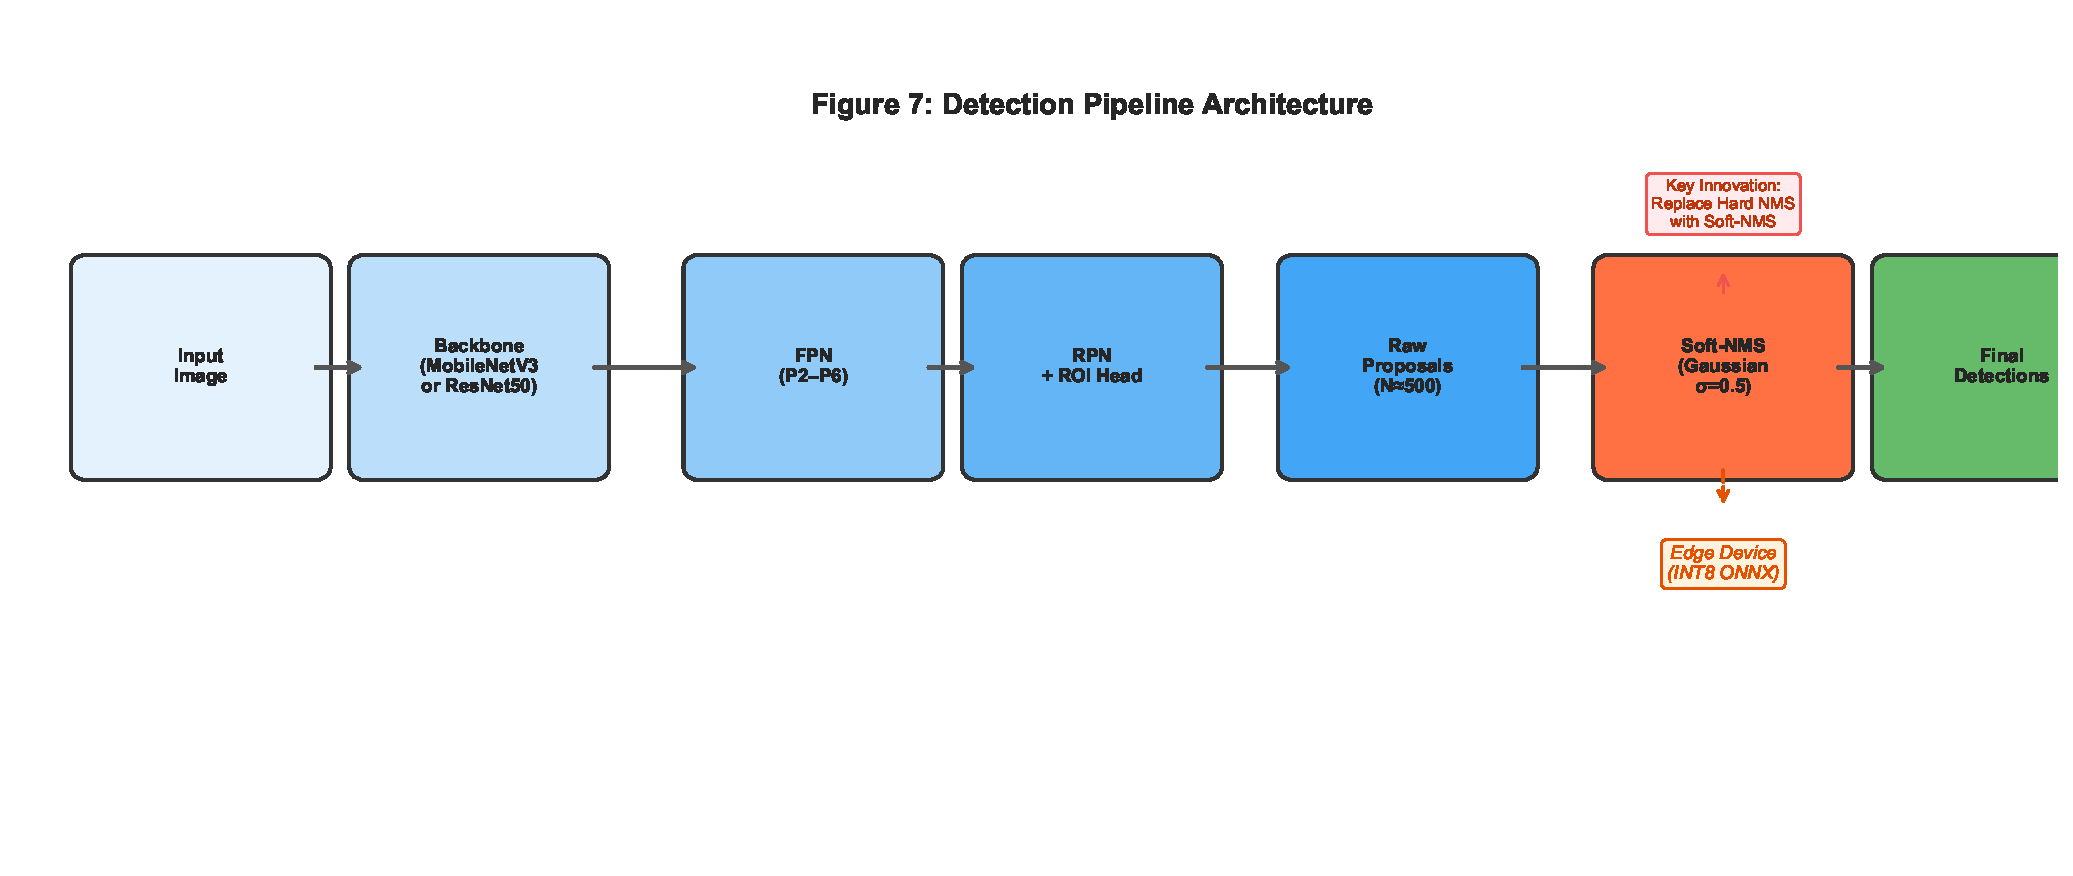
\includegraphics[width=\linewidth]{figures/fig7_architecture.pdf}
\caption{Full detection pipeline architecture.}
\label{fig:architecture}
\end{figure}
